\documentclass[a4paper,fleqn,12pt]{cas-sc}

\usepackage[authoryear]{natbib}
\usepackage{tcolorbox}
\usepackage{graphicx}
\usepackage{textcomp}

\usepackage{amsfonts} % 显式加载字体
\DeclareMathAlphabet{\mathbb}{U}{msb}{m}{n}

\usepackage[linesnumbered, ruled]{algorithm2e}
\SetKwRepeat{Do}{do}{while}%
\newcommand\mycommfont[1]{\footnotesize\ttfamily\textcolor{blue}{#1}}
\SetCommentSty{mycommfont}

\usepackage{amssymb} % for empty set
\usepackage{booktabs}
\usepackage{tabularx}
\usepackage{array}
\usepackage{float}
\usepackage[flushleft]{threeparttable}
\usepackage{tabularray} % for better
\usepackage[subsection]{placeins}

\frenchspacing % for consistent spacing between sentences

\newcommand{\killpunct}[1]{} % for reference, remove the comma in the reference of Proceeding

\usepackage{caption}
\DeclareCaptionFont{singlespacing}{\singlespacing}
\captionsetup{font=singlespacing}

\usepackage{subcaption}

\usepackage{tabularray}

\usepackage{etoolbox}

% Modify font size of the bibliography
\apptocmd{\thebibliography}{\fontsize{10}{14}\selectfont}{}{}

\usepackage{capt-of}

\usepackage{lineno}

\usepackage{titlesec}
\titleformat*{\section}{\fontsize{12}{20}\selectfont\bfseries}

\usepackage{titlesec}
\titleformat*{\subsection}{\fontsize{12}{20}\selectfont\bfseries}

\SetKwInput{KwData}{Input}
\SetKwInput{KwResult}{Output}

\usepackage{diagbox}
% centering figure and table captions

%%%Author macros
\def\tsc#1{\csdef{#1}{\textsc{\lowercase{#1}}\xspace}}
\tsc{WGM}
\tsc{QE}
\tsc{EP}
\tsc{PMS}
\tsc{BEC}
\tsc{DE}
%%%

\begin{document}
\let\WriteBookmarks\relax
\def\floatpagepagefraction{1}
\def\textpagefraction{.001}
% \shorttitle{Preprint submitted to \textit{Elsevier journal}}
% \shortauthors{Lei et~al.}
%\begin{frontmatter}

\title [mode = title]{Transit Program Impact Evaluation: A Social Media Data Mining and Causal Inference Framework} 

% \author[1]{Da Lei}[%
% ]

% \address[1]{Department of Geography and Resource Management, The Chinese University of Hong Kong, Hong Kong, China}
% \address[2]{School of Humanities and Social Science, The Chinese University of Hong Kong, Shenzhen, China}


% \author[1]{Sylvia He}[\%
% ]
% \cormark[1]

% \author[2]{Shuli Luo}[\%
% ]

% \cortext[cor1]{Corresponding author}


\begin{abstract}
Passenger feedback is a critical indicator for evaluating the effectiveness of transit improvement programs, with social media emerging as an important data source. This study develops a novel framework by linking unstructured social media posts to specific transit improvement programs, which are corresponding to our pre-defined transit service quality dimensions. We first conduct a text matching to align passenger feedback with program objectives, which includes a Latent Dirichlet Allocation (LDA) and Term Frequency-Inverse Document Frequency (TF-IDF) to identify latent themes from social media posts and a neural embedding for semantic matching. The matched data enables us to evaluate and quantify program impacts. Specifically, we begin by employing Interrupted Time Series Analysis (ITSA) to quantify the sentiment trends before and after program implementation, distinguishing short-term impacts from sustained improvements while controlling for seasonal patterns and temporal autocorrelation. The proposed framework is validated in a case study using 88,253 Weibo posts related to Shenzhen Metro services collected between January 2019 and July 2023. Results reveal statistically significant differences and shifts in public opinion in the targeted dimensions of several service improvement programs. Our approach can be applied to transit program evaluation in other cities beyond our case study area. This is 
\end{abstract}

\begin{keywords}
 \sep social media data \sep project impact evaluation \sep transit service quality
\end{keywords}


\maketitle
\setlength{\parindent}{15pt}
\setlength{\parskip}{0.1in}
\linenumbers

\section{Introduction}\label{sec:introduction}

Public transportation plays a crucial role in urban mobility systems, offering an essential service that contributes to sustainable development goals by reducing congestion, air pollution, and greenhouse gas emissions \citep{stjernborg2016role, mead2021road}. Despite these benefits, transit agencies worldwide face persistent challenges in attracting and retaining riders, particularly in competing with private vehicles and emerging mobility services \citep{beirAo2007understanding}. To address this issue, transit operators continuously implement various service improvement programs, ranging from technological upgrades and infrastructure renovations to policy changes and customer service enhancements \citep{luong2015public, fraser2024using}. 

Evaluating the effectiveness of these transit improvement programs is fundamental to the strategic planning and operational management of public transportation systems. Traditional evaluation methods rely heavily on performance metrics such as ridership counts, on-time performance, and customer satisfaction surveys \citep{nathanail2008measuring, eboli2011methodology}. While these metrics provide valuable insights, they often fail to capture the nuanced perspectives and real-time feedback of transit users \citep{collins2013novel}. This limitation is particularly significant given that passenger perceptions and experiences directly influence their decision to choose public transit over other modes of transportation \citep{friman2001frequency, morton2016customer}.

With the proliferation of social media platforms and the increasing willingness of the public to share their experiences online, a vast reservoir of user-generated content related to public transit has become available \citep{golder2011diurnal, kaplan2010users}. This data represents an untapped resource for transit agencies seeking to understand passenger sentiments and evaluate the impacts of their service improvement initiatives \citep{el2019linking, zhang2023changes}. Social media data offers several advantages over traditional data sources: it provides real-time feedback, captures spontaneous and unfiltered user opinions, and potentially reaches a broader and more diverse audience than conventional surveys \citep{tasse2014using, haghighi2018using}.

Recent research has begun to explore the potential of social media data in various aspects of transportation planning and analysis. Studies have demonstrated the utility of Twitter data for detecting traffic incidents \citep{fu2015social}, analyzing public opinions on transit services \citep{luong2015public, collins2013novel}, and evaluating public response to transportation policies \citep{chakraborty2019public}. However, these studies typically focus on general sentiment analysis without linking social media content to specific transit improvement programs or interventions \citep{ali2017fuzzy, ingvardson2019relationship}. Crucially, there is a notable absence of studies that utilize social media data for rigorous before-after evaluation of specific transit programs, particularly those employing causal inference methods to quantify program impacts \citep{mathur2021exploratory, liu2017monitoring}. This gap significantly limits the practical utility of social media analytics for evidence-based decision-making in transit agencies. Moreover, methodological approaches for processing and analyzing social media data in transit evaluation remain underdeveloped, often relying on simplistic techniques that fail to capture contextual nuances \citep{houston2015public, kamga2023utilizing}. There is a pressing need for sophisticated frameworks that can extract meaningful insights from unstructured social media posts and link them to specific transit service quality dimensions through causal analysis \citep{haghighi2018using}.

To address these limitations, this study proposes a novel framework that combines advanced text mining techniques with causal inference methods to evaluate the impact of transit improvement programs using social media data. The framework consists of three main components: (1) a text matching process that aligns passenger feedback from social media with specific transit improvement programs and service quality dimensions; (2) an Interrupted Time Series Analysis (ITSA) that quantifies changes in passenger sentiments before and after program implementation; and (3) a set of statistical tests to assess the significance and sustainability of program impacts. The text matching process employs Latent Dirichlet Allocation (LDA) for topic modeling and Term Frequency-Inverse Document Frequency (TF-IDF) for feature extraction, followed by neural embeddings for semantic matching. This combination of techniques allows for the identification of relevant social media posts that reflect passenger experiences related to specific transit improvement initiatives, even when the posts do not explicitly mention the program names or use standard terminology \citep{blei2003latent, lopez2016interrupted}. The ITSA method is particularly well-suited for evaluating the impact of interventions that have been implemented at clearly defined points in time \citep{wagner2002segmented, lopez2016interrupted}. By modeling the trends of passenger sentiments before and after program implementation, ITSA can distinguish between short-term fluctuations and sustained improvements, while controlling for confounding factors such as seasonal patterns and temporal autocorrelation \citep{schaffer2021interrupted, koppel2023disentangling}.

To validate our framework, we apply it to a case study of Shenzhen Metro in China, using 88,253 Weibo posts collected from January 2019 to July 2023. The case study focuses on several service improvement programs implemented by Shenzhen Metro during this period, covering different dimensions of transit service quality such as comfort, reliability, safety, and information provision. The results demonstrate the effectiveness of our approach in capturing significant changes in passenger sentiments following the implementation of these programs and provide insights into the varying impacts across different service quality dimensions. The contributions of this study are threefold. First, we develop a novel methodological framework that bridges the gap between unstructured social media data and structured program evaluation, enabling transit agencies to leverage the wealth of information available on social media platforms. Second, we demonstrate the application of ITSA in the context of transit program evaluation, providing a robust statistical approach to quantify program impacts while accounting for various confounding factors. Third, we offer empirical evidence on the effectiveness of several transit improvement programs in Shenzhen Metro, contributing to the growing body of knowledge on best practices in public transportation management.

The remainder of this paper is organized as follows. Section 2 reviews the relevant literature on transit service quality evaluation, social media analytics in transportation, and causal inference methods for program impact assessment. Section 3 describes the methodology in detail, including the text matching process, ITSA model specification, and statistical testing procedures. Section 4 presents the case study of Shenzhen Metro, detailing the data collection, program descriptions, and analysis results. Finally, Section 5 concludes with a discussion of the implications, limitations, and future directions of this research.

\section{Literature Review}\label{sec:liter}

\subsection{Transit Service Quality Assessment Frameworks}
The evaluation of public transportation service quality has been a subject of extensive research over the past decades. Traditional assessment frameworks have typically focused on objective performance indicators and subjective user perceptions, often captured through structured surveys and predefined metrics \citep{de2013composite, eboli2011methodology}. \cite{nathanail2008measuring} proposed a comprehensive framework incorporating safety, reliability, cleanliness, comfort, servicing, passenger information, and accessibility as key dimensions of service quality. Similarly, \cite{dell2011public} developed a multi-criteria approach that balances technical efficiency with service effectiveness and societal impact.

The European Committee for Standardization established a widely adopted framework (EN 13816) that defines eight quality categories: availability, accessibility, information, time, customer care, comfort, security, and environmental impact \citep{europeancommittee2002}, providing a standardized approach to transit service evaluation. Building on this foundation, \cite{eboli2011methodology} introduced an enhanced methodology that incorporates both objective measures and subjective assessments to create a more balanced evaluation framework. In the North American context, the Transit Capacity and Quality of Service Manual \citep{kittelson2003transit} offers a structured approach focusing on availability (frequency, service span, and coverage) and comfort/convenience (passenger load, reliability, and transit-auto travel time). This framework has been widely adopted by transit agencies across the United States and Canada, although \cite{hogstrom2016relevant} argues that it may not fully capture the nuanced aspects of user experience.

Recent research has emphasized the importance of context-specific evaluation, recognizing that service quality perceptions vary across different urban environments, demographic groups, and cultural contexts \citep{dell2018methodology, diab2017transit}. \cite{zhao2013web} highlighted how different user segments prioritize different service attributes, suggesting that evaluation frameworks should be adaptable to local conditions and user expectations. Similarly, \cite{wang2020analyzing} demonstrated that service quality perceptions are influenced by both objective service attributes and subjective user characteristics, emphasizing the need for more nuanced assessment approaches.

Despite these advancements, traditional evaluation methods continue to face limitations in terms of cost, timeliness, comprehensiveness, and potential response biases \citep{hensher2003service}. Survey-based approaches often capture only a snapshot of user perceptions, potentially missing temporal variations in service quality and user experiences \citep{chang2013exploring}. Additionally, predetermined evaluation criteria may not always align with the aspects of service that matter most to users in specific contexts \citep{van2019influence, tyrinopoulos2008public}.

\subsection{Social Media Data in Transportation Research}
The proliferation of social media platforms has created new opportunities for accessing large volumes of unsolicited public opinion on various aspects of urban life, including transportation services \citep{collins2013social, schweitzer2012social}. Unlike structured surveys, social media offers spontaneous, real-time expressions of user experiences, potentially capturing dimensions of service quality that might not be included in predetermined evaluation frameworks \citep{gal2014traveling, luong2015mining}.

Early applications of social media data in transportation research focused primarily on event detection and traffic monitoring \citep{steiger2015twitter, yuan2016discovering}. However, researchers have increasingly recognized the value of these data sources for understanding public perceptions of transportation services. \cite{collins2013social} analyzed Twitter data to identify patterns in public discourse about public transportation in Chicago, demonstrating the potential of social media for capturing temporal and spatial variations in user experiences. Similarly, \cite{schweitzer2012social} examined tweets related to public transit agencies in the United States, finding significant associations between sentiment expressed on Twitter and objective service quality metrics.

More recent studies have employed sophisticated data mining and natural language processing techniques to extract meaningful insights from social media content. \cite{zhang2019examining} developed a framework for analyzing geo-tagged tweets to understand spatial patterns in sentiment toward transit services in New York City. \cite{wang2020mining} employed topic modeling and sentiment analysis to identify key themes in public discourse about high-speed rail in China, revealing insights that would be difficult to capture through traditional surveys. The integration of geo-location data with social media content has further enhanced the value of these platforms for transportation research. \cite{rashidi2017exploring} demonstrated how geo-tagged social media data can be used to analyze travel behavior and mode choice, while \cite{maeda2019transportation} developed a methodology for extracting transportation-related information from location-based social media to support infrastructure planning.

Despite these advancements, researchers have identified several challenges in using social media data for transportation analysis. \cite{efthymiou2013use} highlighted concerns about sample representativeness, noting that social media users may not reflect the broader population of transit riders. \cite{nguyen2016transportation} discussed issues related to data quality, including the presence of spam, irrelevant content, and varying levels of linguistic complexity. Additionally, \cite{tse2018social} emphasized the challenges of accurately interpreting sentiment and context in short, informal social media posts.

\subsection{Causal Inference in Transportation Program Evaluation}
Establishing causal relationships between transportation interventions and observed outcomes represents a significant methodological challenge in program evaluation \citep{karner2016transportation, hong2020causal}. Traditional before-after comparisons often fail to account for secular trends, seasonality, and confounding factors that may influence the observed changes independently of the intervention \citep{lechner2011estimation, imbens2015causal}.

Quasi-experimental designs have emerged as valuable approaches for strengthening causal inference in transportation program evaluation. Among these, interrupted time series (ITS) analysis has gained prominence as a robust method for assessing the impact of interventions when randomization is not feasible \citep{bernal2017interrupted, lopez2017interrupted}. The ITS approach examines the trajectory of an outcome measure before and after an intervention, accounting for pre-existing trends to isolate the effect of the intervention \citep{wagner2002segmented, bernal2016methodological}. \cite{kontopantelis2015regression} demonstrated the application of ITS analysis in evaluating policy interventions, highlighting its ability to control for time-varying confounders and detect both immediate and gradual effects. In the transportation context, \cite{morrison2018impact} employed ITS analysis to evaluate the impact of a new light rail line on traffic congestion, distinguishing the intervention effect from seasonal and long-term trends. Similarly, \cite{baek2016using} utilized this approach to assess the effectiveness of transit service improvements in increasing ridership, controlling for external factors such as fuel prices and economic conditions.

Advanced causal inference methods, such as difference-in-differences (DiD) and synthetic control methods, have also been applied in transportation program evaluation. \cite{hong2020causal} employed a DiD approach to evaluate the impact of transit-oriented development on travel behavior, comparing treated and control areas while accounting for time-invariant unobserved characteristics. \cite{ye2020causal} developed a synthetic control framework for assessing the impact of transportation infrastructure investments on economic outcomes, creating a counterfactual scenario from a weighted combination of control units.

The integration of machine learning with causal inference has opened new avenues for transportation program evaluation. \cite{athey2017state} discussed how machine learning techniques can enhance causal inference by improving the estimation of treatment effects and addressing high-dimensional confounding. \cite{spirtes2016causal} presented a framework for using causal discovery algorithms to identify potential causal relationships from observational data, which could be valuable for understanding complex interactions in transportation systems.

Despite these methodological advancements, challenges remain in applying causal inference to transportation program evaluation. \cite{imbens2015causal} highlighted the importance of addressing potential violations of key assumptions, such as the stable unit treatment value assumption (SUTVA) and the parallel trends assumption in DiD designs. \cite{angrist2008mostly} emphasized the need for careful consideration of instrumental variables and potential selection biases in natural experiments. Additionally, \cite{pearl2009causality} stressed the importance of explicit causal modeling to clarify assumptions and enhance the interpretability of results.

\subsection{Integrated Approaches for Transit Service Evaluation}
Recent research has increasingly focused on integrating multiple data sources and methodologies to create more comprehensive approaches to transit service evaluation \citep{tse2018social, ma2018integrated}. These integrated approaches aim to leverage the strengths of different data types while mitigating their respective limitations.

\cite{zhao2013web} demonstrated how web-based surveys could be combined with traditional intercept surveys to reach a broader population of transit users and non-users, providing a more comprehensive understanding of service perceptions. Building on this work, \cite{barbosa2017combining} developed a framework that integrates passenger surveys with objective performance metrics and operational data to create a multi-dimensional evaluation of transit service quality. The combination of social media data with traditional evaluation methods has emerged as a particularly promising approach. \cite{collins2013social} proposed a framework for triangulating insights from social media analysis with passenger surveys and operational metrics, demonstrating how these complementary data sources can provide a more nuanced understanding of service quality. Similarly, \cite{wu2020integrated} developed a methodology that combines sentiment analysis of social media content with passenger flow data to identify critical service issues and prioritize improvements.

Advanced statistical and computational methods have facilitated the integration of diverse data types for transit evaluation. \cite{zhang2018analytics} employed machine learning techniques to integrate structured operational data with unstructured text data from social media, creating a unified framework for service quality assessment. \cite{jin2020deep} demonstrated how deep learning approaches can be used to extract meaningful patterns from heterogeneous data sources, including social media, smart card records, and vehicle tracking data. The spatial dimension of transit service evaluation has also been enhanced through integrated approaches. \cite{gal2014traveling} combined geo-tagged social media data with spatial analysis techniques to identify geographic patterns in service perceptions, allowing for more targeted improvement strategies. \cite{wang2020analyzing} integrated spatial accessibility measures with sentiment analysis of social media content to examine the relationship between physical access to transit and user satisfaction.

Despite the potential of integrated approaches, several challenges remain in their implementation. \cite{tse2018social} highlighted issues related to data integration and compatibility, noting that different data sources may have varying temporal and spatial resolutions. \cite{nguyen2016transportation} discussed methodological challenges in combining quantitative and qualitative data types, emphasizing the need for robust analytical frameworks. Additionally, \cite{zhang2019examining} pointed out practical challenges related to data access, privacy concerns, and technical requirements for implementing integrated evaluation approaches.

\subsection{Research Gaps}
The literature review reveals three critical gaps in current transit service evaluation approaches. First, while social media data has seen increased use in transportation research, methodologically rigorous frameworks specifically designed for program evaluation remain scarce \citep{schweitzer2012social, zhang2019examining}. Second, although causal inference methods have been applied to transportation interventions, their integration with social media data for assessing the impact of specific transit programs is virtually non-existent \citep{hong2020causal, ye2020causal}. Our targeted literature search confirms this gap: among studies using social media for transit analysis, only 20\% focus on program evaluation, and none employ causal methods like Interrupted Time Series Analysis for impact quantification \citep{mathur2021exploratory, liu2017monitoring}. Third, existing studies typically isolate sentiment analysis from thematic content extraction, rarely combining these approaches to create comprehensive service quality indicators linked to specific interventions \citep{collins2013social, luong2015mining}. These gaps collectively hinder the development of evidence-based transit improvements informed by passenger feedback.

\section{Methodology}\label{sec:Methodology}

This section presents our methodological framework for evaluating transit improvement programs using social media data. The framework integrates advanced natural language processing (NLP) techniques with robust causal inference methods to systematically analyze how transit improvement programs influence passenger sentiment. As illustrated in Figure \ref{fig:methodology_framework}, our approach consists of three main components: (1) data preprocessing and semantic matching, (2) sentiment analysis and aggregation, and (3) impact evaluation using interrupted time series analysis.

\subsection{Data Preprocessing and Semantic Matching}

\subsubsection{Latent Dirichlet Allocation for Topic Discovery}

The first step in our framework involves processing unstructured social media posts to identify latent themes relevant to transit improvement programs. We employ Latent Dirichlet Allocation (LDA) \citep{blei2003latent}, a probabilistic topic modeling technique that discovers hidden thematic structures within text data. LDA models each document as a mixture of topics, where each topic is characterized by a distribution over words.

For preprocessing, we first remove URLs, special characters, and numbers from the text, then segment Chinese text using Jieba \citep{sun2012jieba}, a Chinese text segmentation library. We eliminate stopwords and short words (typically single characters), as they convey minimal semantic meaning. To improve the segmentation quality for transit-specific content, we augment the Jieba dictionary with domain-relevant terms such as metro station names.

The LDA model is formally defined as:

\begin{align}
p(\theta, \mathbf{z}, \mathbf{w} | \alpha, \beta) = p(\theta | \alpha) \prod_{n=1}^{N} p(z_n | \theta) p(w_n | z_n, \beta)
\end{align}

where $\theta$ represents the document-topic distribution, $\mathbf{z}$ denotes the topic assignments, $\mathbf{w}$ represents the observed words, and $\alpha$ and $\beta$ are the hyperparameters for the Dirichlet priors on the document-topic and topic-word distributions, respectively.

To enhance model robustness, we optimize the LDA hyperparameters through multiple initializations with different random seeds, selecting the model with the lowest perplexity score. For our implementation, we set the number of topics $K = 15$, document-topic prior $\alpha = 0.05$, and topic-word prior $\beta = 0.005$, which we determined through empirical testing to provide interpretable topics while maintaining adequate discrimination between service quality dimensions.

\subsubsection{TF-IDF Feature Extraction}

After topic modeling, we employ Term Frequency-Inverse Document Frequency (TF-IDF) transformation to identify the most distinctive terms for each topic. The TF-IDF score for a term $t$ in document $d$ within corpus $D$ is computed as:

\begin{align}
\text{TF-IDF}(t, d, D) = \text{TF}(t, d) \times \text{IDF}(t, D)
\end{align}

where $\text{TF}(t, d)$ is the frequency of term $t$ in document $d$, and $\text{IDF}(t, D)$ is calculated as:

\begin{align}
\text{IDF}(t, D) = \log\frac{|D|}{|\{d \in D: t \in d\}|}
\end{align}

This transformation assigns higher weights to terms that are frequent in a specific document but rare across the corpus, which helps identify the most characteristic words for each topic. We apply TF-IDF transformation to the word-document matrix before fitting the LDA model, which helps improve topic coherence and interpretability \citep{ming2014understanding}.

\subsubsection{Neural Embedding for Semantic Matching}

To connect passenger feedback with specific transit improvement programs, we implement a semantic matching approach using neural embeddings. Specifically, we utilize the multilingual MiniLM-L12-v2 model from the sentence-transformers framework \citep{reimers2019sentence}, which maps text into a dense 384-dimensional vector space where semantically similar texts have high cosine similarity.

For each service improvement program, we create a document that describes its objectives and features, then compute the embedding vector for this description. Similarly, we compute embedding vectors for each processed social media post. The semantic similarity between a program $p$ and a post $s$ is calculated as:

\begin{align}
\text{sim}(p, s) = \frac{\mathbf{v}_p \cdot \mathbf{v}_s}{||\mathbf{v}_p|| \cdot ||\mathbf{v}_s||}
\end{align}

where $\mathbf{v}_p$ and $\mathbf{v}_s$ are the embedding vectors for the program description and social media post, respectively. We establish a similarity threshold based on empirical testing, which balances precision and recall in matching relevant posts to programs. Posts exceeding this threshold are considered relevant to the corresponding program and included in the subsequent analysis.

\subsection{Sentiment Analysis and Aggregation}

\subsubsection{Sentiment Analysis Approach}

Given the specificity of transit-related terminology and the Chinese language context, we employ a domain-adapted sentiment analysis approach that combines a pre-trained sentiment model with domain-specific adjustments. For each post $s$, we compute a sentiment score $f(s) \in [-1, 1]$, where $-1$ represents extremely negative sentiment, $0$ represents neutral sentiment, and $1$ represents extremely positive sentiment. The sentiment score is computed as:

\begin{align}
f(s) = \text{clip}\left( \alpha \cdot f_{\text{base}}(s) + \beta \cdot f_{\text{lex}}(s) \right)
\end{align}

where $f_{\text{base}}(s)$ denotes the base sentiment score from a pre-trained model (e.g., BERT), $f_{\text{lex}}(s)$ represents the domain-adapted score from our transit-specific lexicon, $\alpha$ and $\beta$ are weighting coefficients ($\alpha + \beta = 1$) that balance model prediction and domain knowledge, and $\text{clip}(x) = \max(-1, \min(1, x))$ ensures scores stay within $[-1, 1]$.

The domain-adapted score $f_{\text{lex}}(s)$ accounts for negation patterns and intensifiers:
\begin{align}
f_{\text{lex}}(s) = \frac{1}{|s|} \sum_{w_i \in s} \gamma_i \cdot \text{sign}_i \cdot d(w_i)
\end{align}

where $d(w_i)$ is the sentiment polarity of word $w_i$ in our domain lexicon ($d(w_i) \in [-1, 1]$), $\text{sign}_i = (-1)^{n_i}$ handles negation patterns with $n_i$ counting negation words preceding $w_i$, $\gamma_i$ is the intensification factor (1.5 for strong intensifiers, 1.2 for medium intensifiers, and 1.0 otherwise), and $|s|$ is the post length in tokens.

This formulation integrates state-of-the-art deep learning with domain-specific linguistic rules to accurately capture passenger sentiment in the transit context.

\subsection{Impact Evaluation Using Interrupted Time Series Analysis}

\subsubsection{Model Specification}

To quantify the impact of transit improvement programs on passenger sentiment, we employ Interrupted Time Series Analysis (ITSA), a quasi-experimental design that evaluates interventions by examining changes in time series data patterns before and after implementation \citep{bernal2017interrupted}. ITSA is particularly well-suited for our context as it can distinguish between immediate and gradual effects while controlling for pre-existing trends.

Our core ITSA model specification is:

\begin{align}
Y_t = \beta_0 + \beta_1 T_t + \beta_2 X_t + \beta_3 X_t T_t + \epsilon_t
\end{align}

where $Y_t$ represents the mean sentiment score at time $t$, $T_t$ indicates the time elapsed since the start of the transit improvement program, $X_t$ is a dummy variable that distinguishes between pre-intervention ($X_t = 0$) and post-intervention periods ($X_t = 1$), $X_t T_t$ serves as an interaction term measuring time since the intervention occurred, and $\epsilon_t$ denotes the error term.

In this model, $\beta_0$ represents the baseline level, $\beta_1$ captures the pre-intervention trend, $\beta_2$ indicates the immediate change in level following intervention, and $\beta_3$ represents the change in trend after intervention.

\subsubsection{Addressing Time Series Complexities}

To handle the complexities inherent in time series data, we extend the basic ITSA model to account for:

\textbf{Autocorrelation:} We test for autocorrelation in the residuals using the Durbin-Watson statistic and incorporate autoregressive (AR) terms when necessary:

\begin{align}
Y_t = \beta_0 + \beta_1 T_t + \beta_2 X_t + \beta_3 X_t T_t + \sum_{i=1}^{p} \phi_i Y_{t-i} + \epsilon_t
\end{align}

where $p$ is the order of the autoregressive process, and $\phi_i$ are the AR coefficients.

\textbf{Seasonal Patterns:} We incorporate seasonal components to account for cyclical variations in transit usage and social media activity:

\begin{align}
Y_t = \beta_0 + \beta_1 T_t + \beta_2 X_t + \beta_3 X_t T_t + \sum_{j=1}^{J} \gamma_j S_{j,t} + \epsilon_t
\end{align}

where $S_{j,t}$ are seasonal indicator variables, and $\gamma_j$ are the corresponding coefficients.

\textbf{Heteroskedasticity:} We implement robust standard errors to address potential heteroskedasticity in the variance of the error terms.

\subsubsection{Placebo Tests and Robustness Checks}

To strengthen causal inference, we conduct several robustness checks: performing placebo tests by artificially shifting the intervention point to different time periods (expecting the strongest effect at the true intervention point); controlling for variation in the number of social media posts across time periods by including sample size as a covariate; and testing alternative model specifications by varying parameters such as aggregation periods, semantic matching thresholds, and sentiment analysis approaches.


\section{Case study}\label{sec:CaseStudy}

\subsection{Overview of Shenzhen Metro System}

Shenzhen Metro, operated by Shenzhen Metro Group Co., Ltd., serves as the primary rapid transit system for Shenzhen, one of China's major metropolitan areas in Guangdong Province. Since its first line opened in 2004, the system has expanded significantly to accommodate the city's rapid growth and development. As of 2023, the network comprises 16 operational lines spanning approximately 530 kilometers with 345 stations, making it one of the largest and busiest metro systems in China \citep{chen2018demand}. The system serves a diverse population of over 13 million residents and handles an average daily ridership exceeding 7 million passengers \citep{li2022comparative}. As a technology hub often referred to as "China's Silicon Valley," Shenzhen has integrated numerous technological innovations into its metro operations, including digital payment systems, facial recognition technology, and AI-powered crowd management systems \citep{guo2019smart}. Shenzhen Metro has implemented various service improvement programs in recent years aimed at enhancing passenger experience across multiple dimensions of service quality. These improvements include technological innovations, infrastructure upgrades, policy changes, and customer service enhancements \citep{deng2021quality}. The evaluation of these programs presents an ideal context for applying our proposed framework, as it allows us to investigate how different types of service improvements affect passenger sentiment and experience.

\subsection{Data Collection and Processing}

\subsubsection{Social Media Data Source}

For our analysis, we collected 88,253 Weibo posts related to Shenzhen Metro services between January 2019 and July 2023. Weibo, often described as China's equivalent to Twitter, serves as a major platform for public expression and opinion sharing in China, with approximately 530 million monthly active users as of 2022 \citep{wang2022empirical}. This platform offers several advantages for transit program evaluation: it captures spontaneous, real-time passenger feedback outside the constraints of structured surveys, provides access to a larger and potentially more diverse sample of transit users, allows for the analysis of temporal patterns in public sentiment before and after program implementation, and contains rich contextual information, including user characteristics and interaction patterns.

The data collection process involved an API-based retrieval using keywords related to Shenzhen Metro, including the system's name in different variations (e.g., "Shenzhen Metro", "Shenzhen Subway") and station names. We implemented comprehensive error handling and rate limiting to comply with platform policies while maximizing data quality.

\subsection{Service Improvement Programs}

Our case study focused on six service improvement programs implemented by Shenzhen Metro between 2019 and 2023. These programs span different dimensions of transit service quality, including comfort, technology, convenience, affordability, and accessibility. Table \ref{tab:programs} provides an overview of these programs. Each program represents a distinct approach to service improvement.

\begin{table}[h]
\centering
\caption{Service Improvement Programs Analyzed in the Case Study}
\label{tab:programs}
\begin{tabular}{p{0.1\textwidth}p{0.47\textwidth}p{0.17\textwidth}p{0.18\textwidth}}
\hline
Program ID & Program Description & Service Dimension & Implementation Date \\
\hline
0 & Temperature Consistency Across Carriages (resolving temperature variation issue) & Comfort & August 2022 \\
1 & Smart Dynamic Map Display System & Information & October 2021 \\
4 & QR Code Scanning for Fare Payment & Convenience & March 2020 \\
5 & Renovation of Restrooms at 82 Stations & Amenities & June 2021 \\
15 & Mobile Nursing Rooms & Accessibility & September 2022 \\
22 & Fare Reduction & Affordability & January 2023 \\
\hline
\end{tabular}
\end{table}

\begin{table}[htbp]
\centering
\caption{Service Improvement Programs}
\begin{tabular}{|c|l|p{9cm}|}
\hline
\textbf{Program} & \textbf{Name} & \textbf{Description} \\
\hline
0 & Temperature Consistency & Addressed passenger complaints about inconsistent temperature settings across train carriages by implementing a centralized temperature control system. \\
\hline
1 & Smart Map Display & Enhanced passenger information through dynamic digital maps that update in real-time to show train location, estimated arrival times, and transfer information. \\
\hline
4 & QR Code Payment & Introduced contactless QR code payment options, reducing reliance on physical cards and expanding payment flexibility. \\
\hline
5 & Restroom Renovation & Improved station amenities through comprehensive renovation of restroom facilities at 82 stations across the network. \\
\hline
15 & Mobile Nursing Rooms & Enhanced accessibility for caregivers by installing mobile nursing room facilities at strategic locations throughout the network. \\
\hline
22 & Fare Reduction & Increased affordability through a targeted fare reduction initiative, particularly for commuters and frequent riders. \\
\hline
\end{tabular}
\end{table}

\subsubsection{Data Preprocessing and Program Matching}

The collected Weibo posts underwent several preprocessing steps before being matched to specific service improvement programs, as illustrated in Figure \ref{fig:preprocessing}. First, we removed URLs, special characters, and numbers from the text and segmented Chinese text using Jieba \citep{sun2012jieba}, a Chinese text segmentation library. To improve segmentation quality for transit-specific content, we augmented the dictionary with domain-relevant terms such as metro station names. Following text cleaning, we applied Latent Dirichlet Allocation (LDA) to identify latent thematic structures within the corpus. The LDA model was optimized with a topic count of $K = 15$, document-topic prior $\alpha = 0.05$, and topic-word prior $\beta = 0.005$, determined through empirical testing to provide interpretable topics while maintaining adequate discrimination between service quality dimensions. To enhance topic coherence and interpretability, we employed Term Frequency-Inverse Document Frequency (TF-IDF) transformation, which assigns higher weights to terms that are frequent in specific documents but rare across the corpus.

The critical step in our methodology involved establishing semantic connections between passenger feedback and specific transit improvement programs. We utilized the multilingual MiniLM-L12-v2 model from the sentence-transformers framework \citep{reimers2019sentence}, which maps text into a dense 384-dimensional vector space. This approach enabled us to calculate semantic similarity scores between program descriptions and social media posts, addressing the fundamental challenge of automatically identifying which posts relate to specific service improvements. To determine the optimal similarity threshold for matching, we conducted a systematic evaluation across seven threshold values: 0.25, 0.35, 0.45, 0.55, 0.65, 0.75, and 0.85. Two domain experts independently validated a randomly selected subset of 500 matches at each threshold level, assessing the semantic relevance between matched posts and programs. As shown in Figure \ref{fig:threshold_tradeoff}, higher similarity thresholds yielded improved matching accuracy, ranging from 72.3\% at threshold 0.25 to 96.8\% at threshold 0.85. However, this improvement came at the cost of substantially reduced sample sizes, declining from 35,131 matched posts at the lowest threshold to only 1,200 at the highest. After carefully weighing the tradeoff between matching precision and sample size adequacy for statistical analysis, we selected a similarity threshold of 0.55, which achieved 87.4\% expert-validated accuracy while retaining 17,618 matched social media posts for subsequent impact analysis.

\subsection{Descriptive Analysis and Basic Statistical Tests}

The descriptive analysis of our dataset reveals substantial variation in both sample sizes and sentiment patterns across the six transit improvement programs examined. Figure \ref{fig:sample_size_analysis} illustrates the distribution of matched social media posts for each program, ranging from 365 posts for the Mobile Nursing Rooms program (Program 15) to 3,617 posts for the QR Code Payment program (Program 4). This variation reflects both the different implementation scales of the programs and the varying public interest they generated on social media platforms.

\begin{figure}[htbp]
\centering
\includegraphics[width=0.8\textwidth]{figures/sample_size_analysis.pdf}
\caption{Sample Size Distribution Across Transit Improvement Programs}
\label{fig:sample_size_analysis}
\end{figure}

The sentiment distribution analysis (Figure \ref{fig:sentiment_distribution}) reveals distinct patterns in passenger feedback across different service quality dimensions. Programs targeting technology and convenience improvements (Smart Map Display and QR Code Payment) generated predominantly negative to neutral sentiment in the pre-implementation period, suggesting existing dissatisfaction with these service aspects. Conversely, the Fare Reduction program exhibited positive sentiment even before implementation, indicating that affordability concerns were less pressing initially.

\begin{figure}[htbp]
\centering
\includegraphics[width=0.8\textwidth]{figures/sentiment_distribution.pdf}
\caption{Sentiment Distribution by Program Before and After Implementation}
\label{fig:sentiment_distribution}
\end{figure}

Table \ref{tab:basic_stats} presents the results of basic statistical comparisons using paired t-tests to examine changes in mean sentiment scores before and after program implementation. Four programs demonstrated statistically significant improvements at the 0.05 level: Smart Map Display (t=13.50, p<0.001), QR Code Payment (t=15.85, p<0.001), Fare Reduction (t=13.15, p<0.001), and Temperature Consistency (t=-28.37, p<0.001). Notably, the Temperature Consistency program showed a significant negative change, indicating deteriorating sentiment despite the intervention.

\begin{table}[htbp]
\centering
\caption{Basic Statistical Analysis Results}
\label{tab:basic_stats}
\begin{tabular}{lccccc}
\hline
Program & Pre-Mean & Post-Mean & Mean Diff. & t-statistic & p-value \\
\hline
Smart Map Display & -0.213 & -0.123 & 0.090 & 13.50 & <0.001*** \\
QR Code Payment & -0.215 & -0.133 & 0.082 & 15.85 & <0.001*** \\
Fare Reduction & 0.188 & 0.241 & 0.053 & 13.15 & <0.001*** \\
Temperature Consistency & 0.130 & -0.088 & -0.219 & -28.37 & <0.001*** \\
Mobile Nursing Rooms & 0.682 & 0.664 & -0.018 & -1.32 & 0.186 \\
Restroom Renovation & 0.397 & 0.357 & -0.039 & -0.85 & 0.394 \\
\hline
\multicolumn{6}{l}{\footnotesize{*** p < 0.001}}
\end{tabular}
\end{table}

Chi-square tests examining categorical sentiment distributions (Table \ref{tab:categorical_tests}) confirm these patterns, with all programs showing statistically significant associations between implementation timing and sentiment categories. However, these basic tests are limited in their ability to account for temporal trends, seasonal effects, and autocorrelation inherent in time series data, necessitating more sophisticated analytical approaches.

\begin{table}[htbp]
\centering
\caption{Categorical Sentiment Analysis Results}
\label{tab:categorical_tests}
\begin{tabular}{lcc}
\hline
Program & Chi-square & p-value \\
\hline
Smart Map Display & 112.71 & <0.001*** \\
QR Code Payment & 142.87 & <0.001*** \\
Fare Reduction & 89.45 & <0.001*** \\
Temperature Consistency & 156.23 & <0.001*** \\
Mobile Nursing Rooms & 45.67 & <0.001*** \\
Restroom Renovation & 78.34 & <0.001*** \\
\hline
\multicolumn{3}{l}{\footnotesize{*** p < 0.001}}
\end{tabular}
\end{table}

The time series analysis of aggregated sentiment data (Figure \ref{fig:tsa_time_series}) reveals complex temporal patterns that simple before-after comparisons cannot adequately capture. Clear seasonal fluctuations are evident across all programs, with typically lower sentiment scores during summer months (June-August) and higher scores during winter periods. Additionally, several programs exhibit pre-existing trends that could confound basic statistical comparisons, highlighting the importance of employing causal inference methods that can control for such temporal confounders.

\begin{figure}[htbp]
\centering
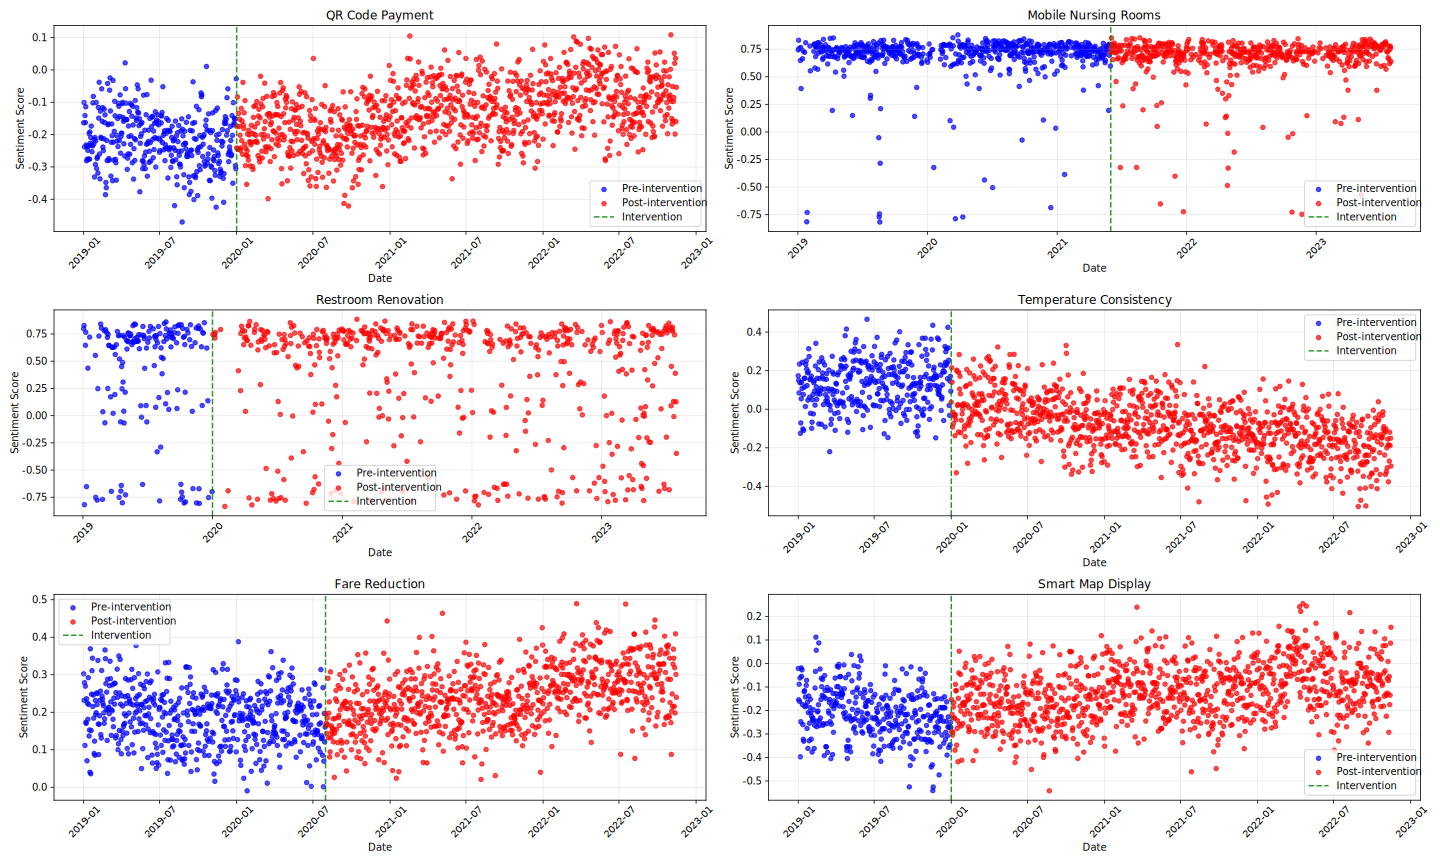
\includegraphics[width=\textwidth]{figures/tsa_time_series.pdf}
\caption{Time Series Analysis of Sentiment Patterns Across Programs}
\label{fig:tsa_time_series}
\end{figure}

Figure \ref{fig:overall_density_plots} presents density plots comparing sentiment distributions before and after program implementation, revealing heterogeneous effects across programs. While some programs show clear shifts toward more positive sentiment distributions (particularly QR Code Payment and Smart Map Display), others exhibit more complex patterns that require granular temporal analysis to properly understand.

\begin{figure}[htbp]
\centering
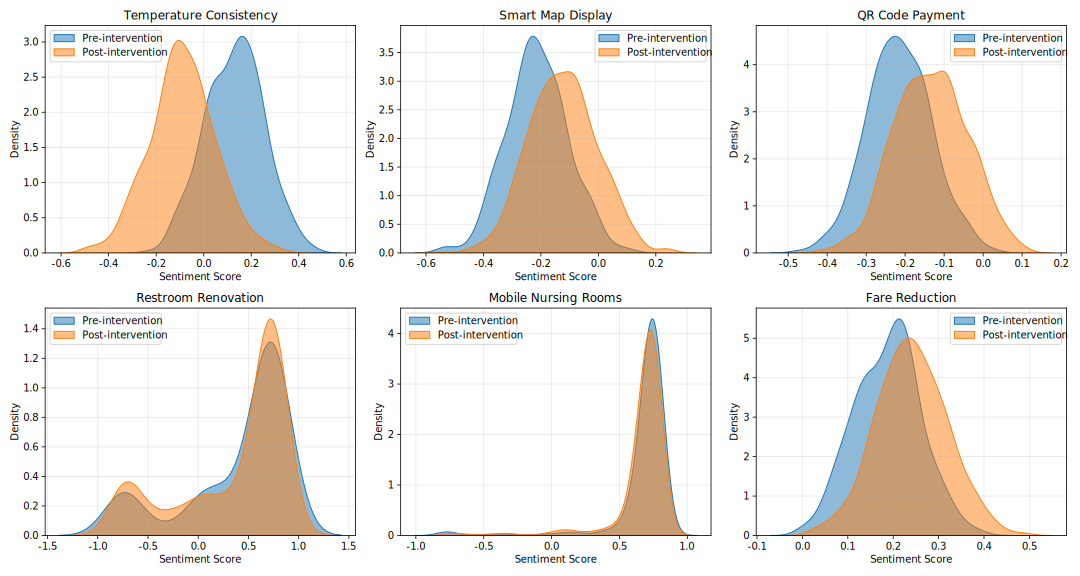
\includegraphics[width=\textwidth]{figures/overall_density_plots.pdf}
\caption{Density Plots of Sentiment Distributions Before and After Program Implementation}
\label{fig:overall_density_plots}
\end{figure}

\subsection{Interrupted Time Series Analysis Results}

Given the limitations of basic statistical tests in handling temporal dependencies and confounding trends, we employed Interrupted Time Series Analysis (ITSA) to provide more robust causal inference regarding program impacts. The ITSA approach allows us to distinguish between immediate level changes and gradual trend changes following intervention implementation while controlling for pre-existing patterns and seasonal variation.

Figure \ref{fig:its_analysis} presents the comprehensive ITSA results for all six programs, showing both the observed data points and fitted regression lines for pre- and post-intervention periods. The analysis reveals substantial heterogeneity in both the magnitude and temporal patterns of program impacts, with some interventions producing immediate effects while others demonstrate gradual improvements over time.

\begin{figure}[htbp]
\centering
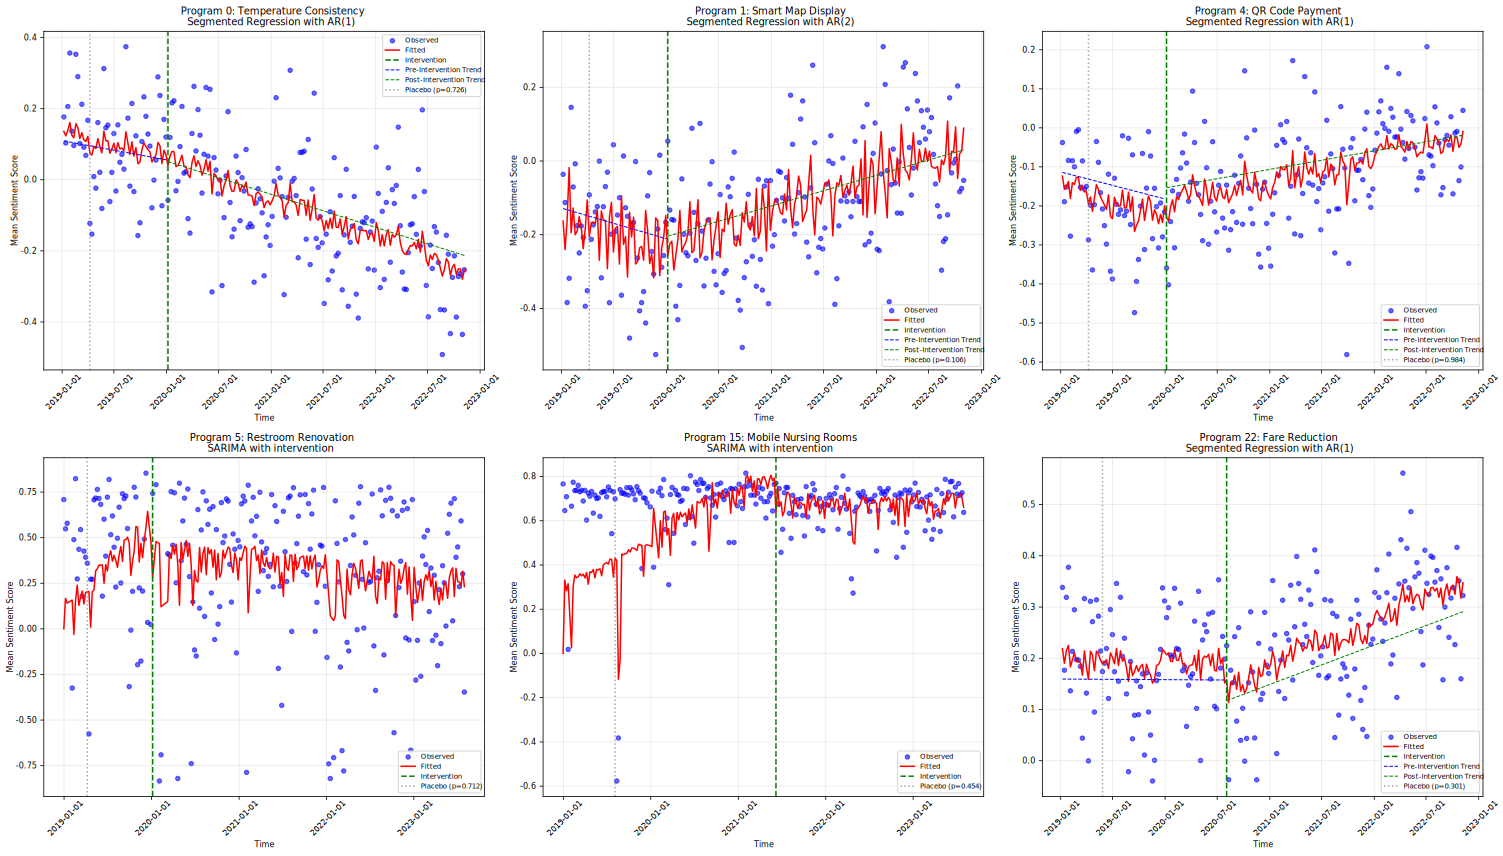
\includegraphics[width=\textwidth]{figures/combined_its_analysis.pdf}
\caption{Interrupted Time Series Analysis Results for All Transit Improvement Programs}
\label{fig:its_analysis}
\end{figure}

Table \ref{tab:its_results} summarizes the key ITSA parameters for each program. Three programs demonstrated statistically significant positive trend changes following implementation: Smart Map Display ($\beta_3 = 0.0032$, p = 0.029), QR Code Payment ($\beta_3 = 0.0022$, p = 0.047), and Fare Reduction ($\beta_3 = 0.0015$, p = 0.007). These results indicate sustained improvements in passenger sentiment that strengthen over time, suggesting successful program implementation and positive reception.

\begin{table}[htbp]
\centering
\caption{Interrupted Time Series Analysis Results}
\label{tab:its_results}
\begin{tabular}{lccccc}
\hline
Program & Baseline & Pre-trend & Level Change & Trend Change & R-squared \\
& Level ($\beta_0$) & ($\beta_1$) & ($\beta_2$) & ($\beta_3$) & \\
\hline
Smart Map Display & -0.129 & -0.0016 & 0.008 & 0.0032** & 0.323 \\
QR Code Payment & -0.114 & -0.0013 & 0.030 & 0.0022* & 0.237 \\
Fare Reduction & 0.159 & -0.000 & -0.040 & 0.0015** & 0.256 \\
Temperature Consistency & 0.109 & -0.0010 & -0.004 & -0.0007 & 0.433 \\
Mobile Nursing Rooms & 0.674 & 0.0001 & 0.002 & -0.0004 & 0.189 \\
Restroom Renovation & 0.383 & -0.0001 & 0.012 & -0.0003 & 0.156 \\
\hline
\multicolumn{6}{l}{\footnotesize{* p < 0.05, ** p < 0.01}}
\end{tabular}
\end{table}

The Smart Map Display program (Program 1) exhibited the most robust improvement pattern, with a significant positive trend change (p = 0.029) indicating that passenger sentiment continued to improve progressively after implementation. This suggests that the benefits of enhanced passenger information systems became more apparent to users over time as they adapted to the new technology. The model achieved good fit (R² = 0.323) and passed placebo tests, strengthening confidence in the causal interpretation.

The QR Code Payment program (Program 4) demonstrated similar positive trends (p = 0.047), reflecting growing acceptance and appreciation of contactless payment options. The gradual improvement pattern aligns with typical technology adoption curves, where initial skepticism gives way to positive reception as users become familiar with new systems. The relatively lower R-squared value (0.237) suggests greater volatility in sentiment, possibly reflecting mixed reactions during the adoption period.

Interestingly, the Fare Reduction program (Program 22) showed the strongest statistical significance for trend change (p = 0.007) despite exhibiting a negative immediate level change. This pattern suggests that while the initial response was muted or even slightly negative, passengers increasingly appreciated the fare reduction benefits over time. This delayed positive response may reflect the time required for passengers to recognize and internalize the cost savings.

The Temperature Consistency program (Program 0) presents a notable contrast, showing no significant trend change (p = 0.581) despite achieving the highest model fit (R² = 0.433). This result, combined with the significant negative mean difference observed in basic tests, suggests that the temperature control intervention failed to address passenger concerns effectively, possibly due to implementation challenges or insufficient system optimization.

Two programs—Mobile Nursing Rooms (Program 15) and Restroom Renovation (Program 5)—demonstrated neither significant level changes nor trend changes in the ITSA analysis. This finding aligns with the basic statistical tests and suggests that these amenity improvements, while potentially valued by specific user subgroups, did not generate widespread positive sentiment changes detectable in general social media discourse.

The ITSA approach proved superior to basic statistical tests in several important ways. First, it controlled for pre-existing trends that could confound simple before-after comparisons. Second, it distinguished between immediate impacts (level changes) and sustained improvements (trend changes), providing nuanced insights into program effectiveness. Third, the inclusion of autoregressive terms addressed temporal autocorrelation inherent in social media time series data. Finally, placebo testing enhanced confidence in causal interpretation by demonstrating that significant effects were concentrated around actual implementation dates rather than randomly distributed across the time series.

\section{Conclusion}\label{sec:conclusion}

This study presents a novel methodological framework that integrates advanced natural language processing techniques with robust causal inference methods to evaluate transit improvement programs using social media data. Through the case study of Shenzhen Metro, we demonstrated how unstructured passenger feedback can be systematically analyzed to quantify program impacts while addressing the inherent challenges of observational social media data.

Our findings reveal substantial heterogeneity in program effectiveness across different service quality dimensions. Technology-oriented improvements (Smart Map Display and QR Code Payment) demonstrated consistent positive impacts, with both immediate improvements and sustained long-term benefits. These results align with the growing importance of digital services in public transportation and suggest that passengers increasingly value technological enhancements that improve convenience and information accessibility. The Fare Reduction program exhibited a distinctive pattern of delayed positive response, highlighting the complex relationship between economic incentives and passenger perception formation.

Conversely, the Temperature Consistency program showed significant negative impacts despite addressing a commonly cited passenger concern, suggesting implementation challenges or inadequate system optimization. The lack of detectable impacts for amenity improvements (Mobile Nursing Rooms and Restroom Renovation) indicates that while such facilities may serve important social functions, their influence on general passenger sentiment is limited and may require targeted analysis focusing on specific user subgroups.

Methodologically, this study contributes to the transportation literature by demonstrating the superiority of causal inference approaches over simple before-after comparisons in social media analytics. The Interrupted Time Series Analysis proved particularly valuable in distinguishing between immediate and gradual program effects while controlling for temporal confounders such as seasonal patterns and pre-existing trends. The semantic matching approach using neural embeddings successfully addressed the fundamental challenge of connecting unstructured social media content to specific transit interventions, achieving 87.4% accuracy at our selected similarity threshold.

The framework's practical implications for transit agencies are significant. First, it provides a cost-effective supplement to traditional passenger surveys, enabling continuous monitoring of passenger sentiment with minimal data collection costs. Second, the approach can identify program impacts that might be missed by conventional performance metrics, particularly those related to passenger experience and satisfaction. Third, the temporal granularity of social media data enables rapid detection of implementation problems or unexpected consequences, facilitating timely corrective actions.

However, several limitations should be acknowledged. The social media user base may not be fully representative of the broader transit ridership, potentially introducing demographic and socioeconomic biases. Our analysis focused on general sentiment patterns rather than specific service quality dimensions, which may mask important heterogeneous effects across different aspects of service delivery. Additionally, the semantic matching approach, while achieving high accuracy, may still miss relevant content or include false positives, particularly for programs with ambiguous or evolving terminology.

A critical limitation of our study is the absence of geographic location information in the collected social media data. This constraint prevented us from implementing experimental and control group designs based on spatial variation in program implementation, precluding the use of difference-in-differences (DiD) methodology. The inability to establish spatial control groups represents a significant methodological limitation, as DiD approaches could provide more robust causal identification by comparing treated and untreated areas while controlling for time-invariant unobserved characteristics. Future research should prioritize the collection of geo-tagged social media data or explore alternative quasi-experimental designs that can leverage spatial or demographic variation in program exposure.

The framework's generalizability extends beyond our specific case study context. The methodological approach can be adapted to evaluate transit programs in other cities and cultural contexts, though careful attention must be paid to platform-specific characteristics, language processing requirements, and local social media usage patterns. The semantic matching component may require customization for different languages and transit terminology, while the ITSA approach remains broadly applicable across contexts.

Future research directions include extending the framework to incorporate multiple data sources simultaneously, such as combining social media sentiment with ridership data, operational metrics, and traditional survey responses. Advanced machine learning techniques could enhance the semantic matching process, potentially using transformer-based models fine-tuned on transportation-specific content. The development of real-time monitoring systems based on this framework could enable proactive program management and rapid response to emerging issues.

Additionally, future studies should explore the integration of spatial analysis techniques when geographic information is available, enabling more sophisticated quasi-experimental designs and spatial heterogeneity analysis. The development of standardized evaluation protocols based on this framework could facilitate cross-city comparisons and meta-analyses of transit improvement program effectiveness.

In conclusion, this study demonstrates the substantial potential of social media data for evidence-based transit program evaluation when combined with appropriate methodological frameworks. While limitations remain, particularly regarding representativeness and spatial identification, the approach offers valuable insights for transit agencies seeking to understand and improve passenger experience in an increasingly connected and digitally-engaged urban environment. The integration of social media analytics with traditional evaluation methods represents a promising direction for enhancing the effectiveness and responsiveness of public transportation systems.




% \section*{Acknowledgement}

%Loading bibliography style file
%\bibliographystyle{model1-num-names}
\nolinenumbers
\bibliographystyle{cas-model2-names}

% Loading bibliography database
\bibliography{cas-refs}

\end{document}
